\section{Glance Gitlab integration}
\label{sec:glance-gitlab-integration}

As already said before, the Glance Phase 0 originated from the need to have an automatic creation of Gitlab repositories for each Analysis or publication. So Phase 0 interface has some buttons that triggers the communication with Gitlab.

A basic structure is already set in Gitlab to store the groups related to an Analysis. The main Gitlab group is called atlas-physics-office and it stores many subgroups. Each of those subgroups belong to a leading group, for example: Higgs and Exotics.

\begin{figure}[ht!]
  \centering
  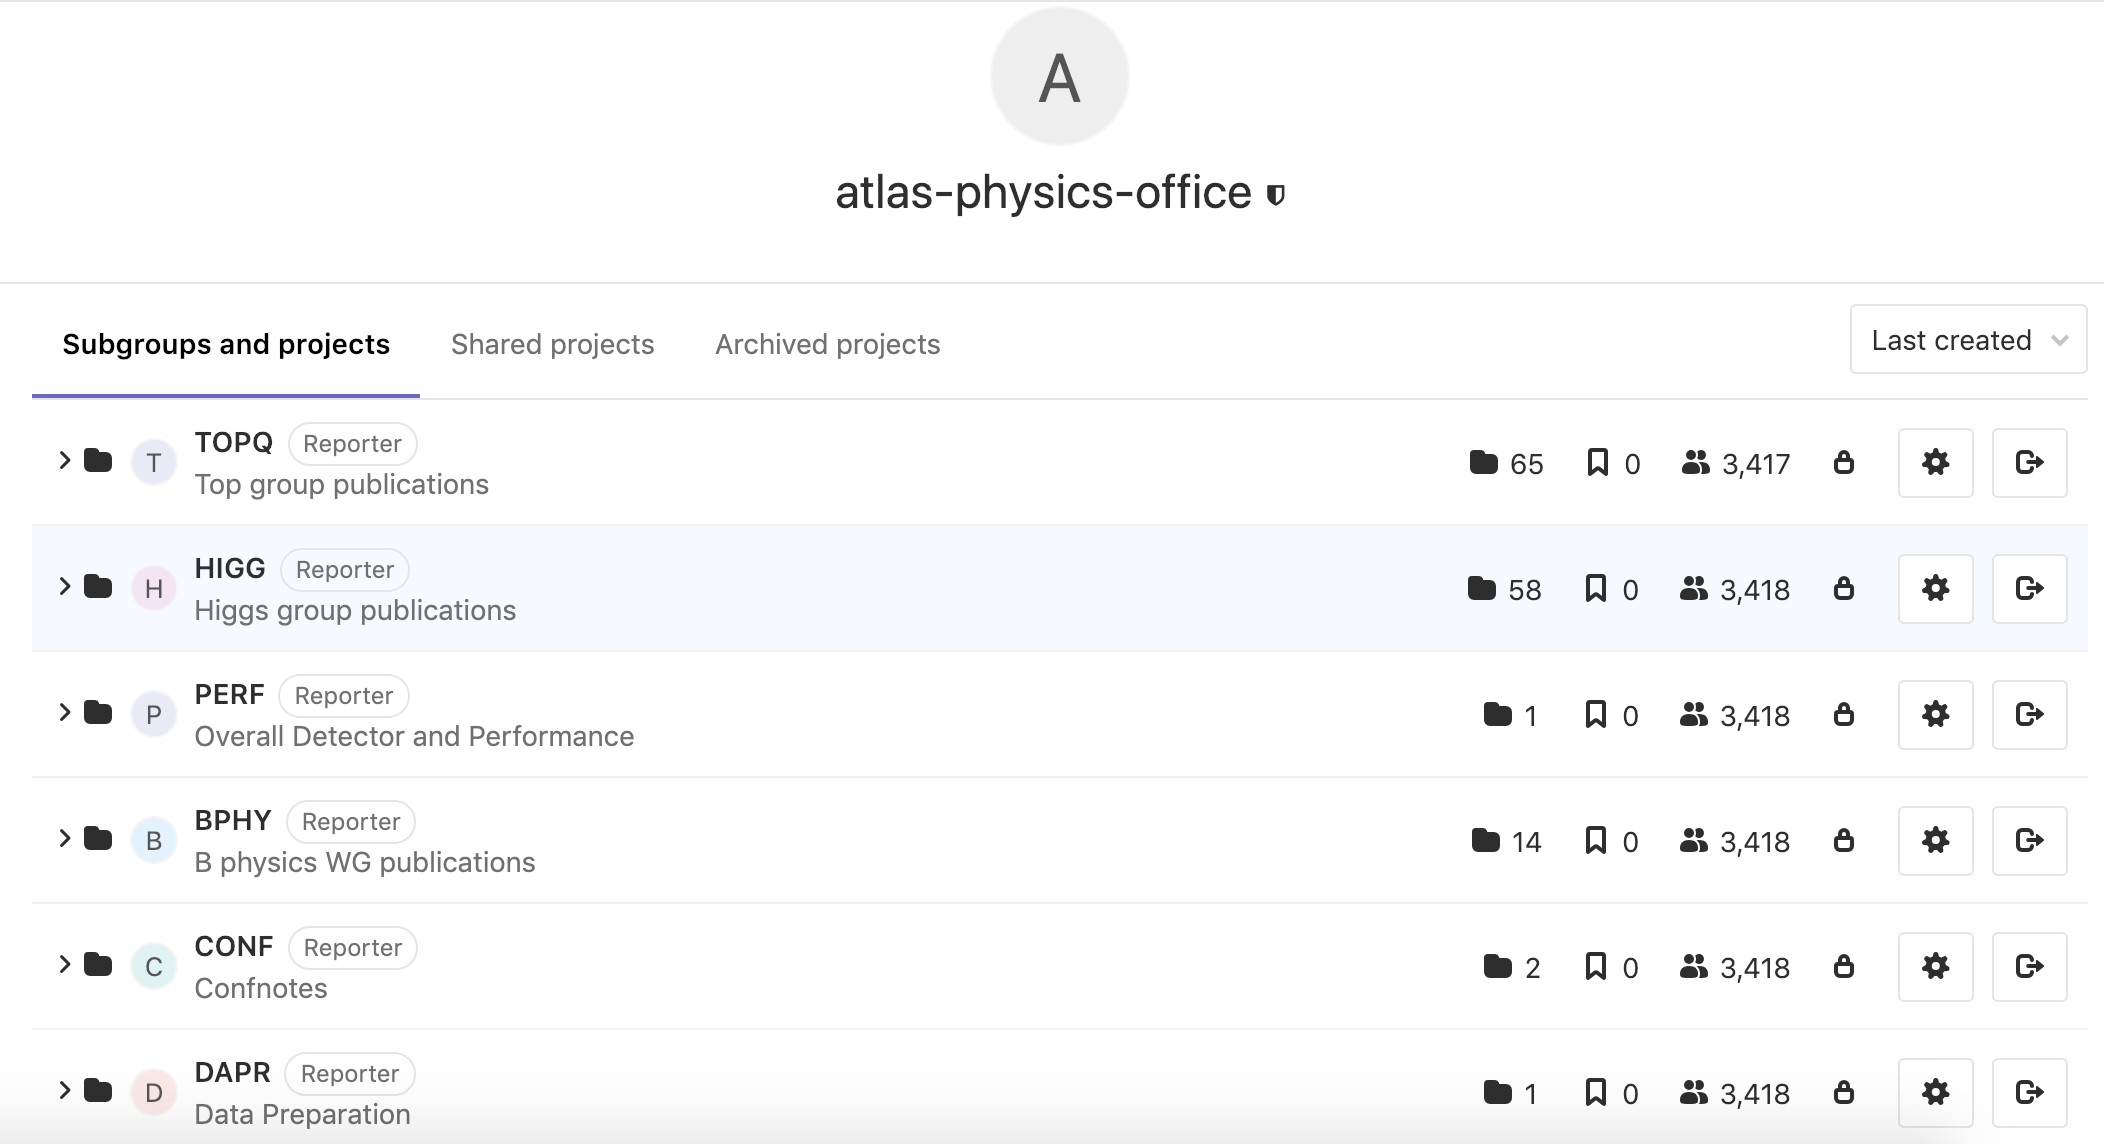
\includegraphics[width=0.9\textwidth]{po-lead-groups-tree.png}
  \caption{Screenshot of leading groups Gitlab infrastructure.}
  \label{fig:po-lead-groups-tree}
\end{figure}

When a Phase 0 entry is created through Glance, a group with its reference code is automatically created containing the first internal note repository. The content of this repository's first commit is get from a source repository with file templates called atlaslatex, also inside atlas-physics-office group. Glance is responsible to substitute the variables in all the file templates according to the metadata inserted when creating the entry in the system. After the commit, Glance automatically unprotects the master branch, creates the protected PO-ready branch an also created PO-Publication label. The last thing done in this first integration is to set the developer permission to the Analysis Team egroup.

Another Glance and Gitlab integration happens when Phase 0 finished or it is skipped, proceeding to Paper, CONF or PUB note Phase 1. When this happens, Glance automatically creates a configured repository inside the Analysis group belonging to the respective publication. It is also possible to add one or more additional internal note repositories at any time.

\begin{figure}[ht!]
  \centering
  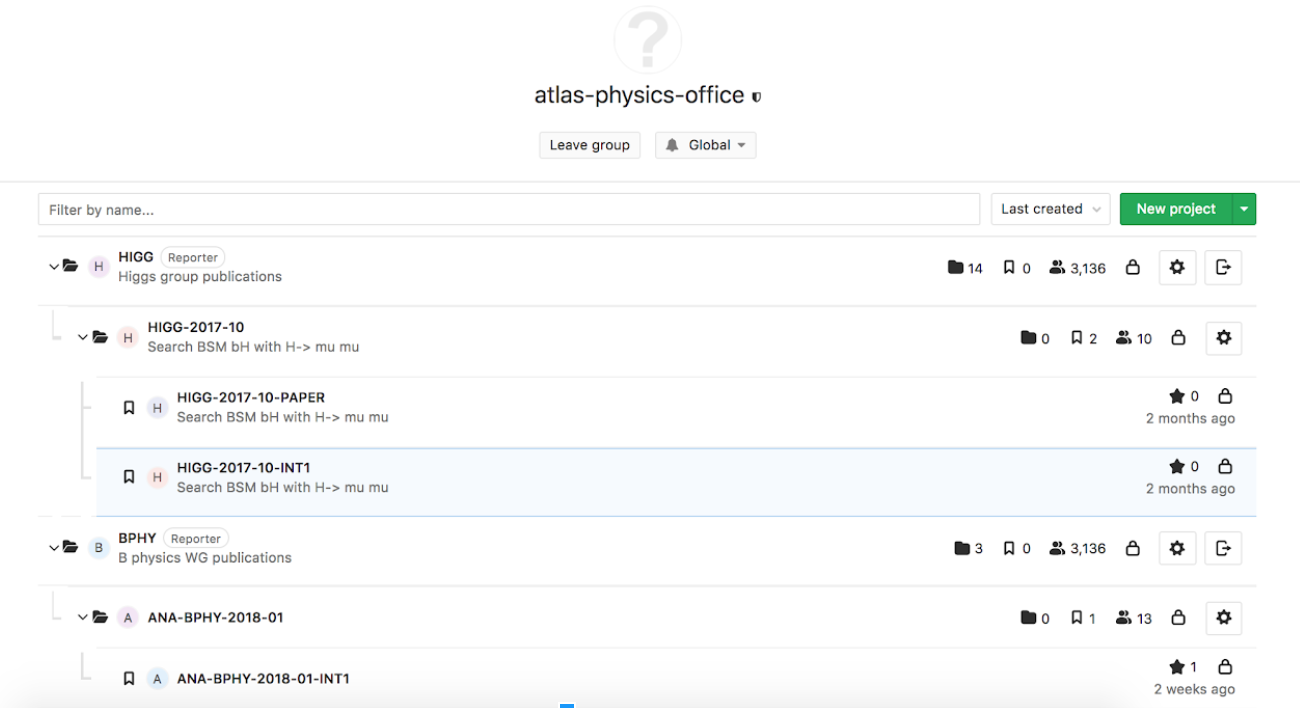
\includegraphics[width=0.9\textwidth]{po-ana-tree.png}
  \caption{Screenshot of Analysis Phase 0 groups Gitlab infrastructure.}
  \label{fig:po-ana-tree}
\end{figure}